 \documentclass[11pt,a4paper]{article}
\usepackage[latin1]{inputenc}
\usepackage{cite}
\usepackage{lmodern}
\usepackage{lipsum}
\usepackage[export]{adjustbox}
\usepackage{amsmath}
\usepackage{amsfonts}
\usepackage{amssymb}
\usepackage{graphicx}
\usepackage{subcaption}
\usepackage{marginnote}
\usepackage{verbatim}
\usepackage{color}   %May be necessary if you want to color links
\usepackage{hyperref}
\hypersetup{
    colorlinks=true, %set true if you want colored links
    linktoc=all,     %set to all if you want both sections and subsections linked
    linkcolor=blue,  %choose some color if you want links to stand out
}
\usepackage[bottom]{footmisc}
\usepackage[top=1.5cm, bottom=3cm, outer=2cm, inner=2cm, heightrounded, marginparwidth=3cm, marginparsep=3cm]{geometry}
\usepackage{listings}
\usepackage{color}

\definecolor{dkgreen}{rgb}{0,0.6,0}
\definecolor{gray}{rgb}{0.5,0.5,0.5}
\definecolor{mauve}{rgb}{0.58,0,0.82}

\lstset{frame=tb,
	language=Python,
	aboveskip=3mm,
	belowskip=3mm,
	showstringspaces=false,
	columns=flexible,
	basicstyle={\small\ttfamily},
	numbers=none,
	numberstyle=\tiny\color{gray},
	keywordstyle=\color{blue},
	commentstyle=\color{dkgreen},
	stringstyle=\color{mauve},
	breaklines=true,
	breakatwhitespace=true,
	tabsize=3
}
%\author{Rachana(PH15B007)\\Guide:Prof.Arul Lakshminarayan}
\title{Entanglement Dynamics in Randomly Kicked 1D Ising Model}

\begin{document}
\maketitle
\tableofcontents
\section{Kicked  Ising Hamiltonian }
Consider a 1-D spin chain with interactions only along the x-axis, and a pulsed magnetic field along z-axis which acts on all spins at once. This model is referred to as the kicked Ising model.The Hamiltonian for the kicked Ising model with periodic boundary conditions imposed is given by:
		 \begin{equation}\label{key}
		 H(t)= \sum_{j=1}^{L}\sigma_{j}^{x} \sigma_{j+1}^{x} + \sum_{k=-\infty}^{\infty}\delta(k-\dfrac{t}{T})\sum_{j=1}^{L}\sigma_{j}^{z}
		 \end{equation}
		 Here $T$ is the time period after which the kicks are applied to the Ising chain. 
		
Deriving time evolution operator for Floquet system:

The Schr\"{o}dinger equation for this kicked Ising model is given by (let $\sum_{j=1}^{L}\sigma_{j}^{x} \sigma_{j+1}^{x}  = H_{0} $, $\sum_{j=1}^{L}\sigma_{j}^{z} = H_{1}$ and $\delta_{T}(t) =  \sum_{k=-\infty}^{\infty}\delta(k-\dfrac{t}{T})$),

\begin{equation}
i \hbar \dfrac{\partial}{\partial t}|\psi\rangle = H_{0}|\psi\rangle + H_{1} \delta_{T}(t) |\psi\rangle
\end{equation}

 In the time interval between two consecutive kicks, only $H_{0}$ contributes to the unitary operator. So, therefore we define:
\begin{equation}
U_{after} = \exp(-iH_{0}T/\hbar)
\end{equation}

Here $U_{after}$ is the unitary operator that acts between consecutive kicks. Now, in order to find the unitary evolution operator at the time of the kick, we integrate the Schr\"{o}dinger equation over an infinetisimal time interval about $t = T $. This eliminates the $H_{0}$ part and we will be left with:
\begin{equation}
i\hbar \dfrac{\partial}{\partial t} |\psi\rangle = H_{1}\delta_{T}(t) |\psi\rangle
\end{equation}

Solving by integrating over an infinitesimal time interval $\epsilon$, we get (and setting $\hbar = 1$):
\begin{align}
i \log(\dfrac{|\psi(T+\epsilon)\rangle}{|\psi(T-\epsilon)\rangle}) &= \int_{T-\epsilon}^{T+\epsilon} H_{1}\delta_{T}(t)\\
|\psi(T+\epsilon)\rangle &= \exp(-iH_{1}T)|\psi(T-\epsilon)\rangle 
\end{align}
This gives the time evolution operator at the time of kicking to be:
\begin{equation}
U_{kick} = \exp(-iH_{1}T)
\end{equation}

In this study, we consider the evolution with the time period $\dfrac{\pi}{4}$\cite{PhysRevA.91.022318}. Hence the overall unitary operator driving the system for one time period would be:
		 
		 \begin{equation}
		 U = U_{after}U_{kick} = \exp(-i\dfrac{\pi}{4}\sum_{j=1}^{L}\sigma_{j}^{x} \sigma_{j+1}^{x})  \exp(-i\dfrac{\pi}{4}\sum_{j=1}^{L}\sigma_{j}^{z})
		 \end{equation}
		 
		 \begin{figure}[h!]
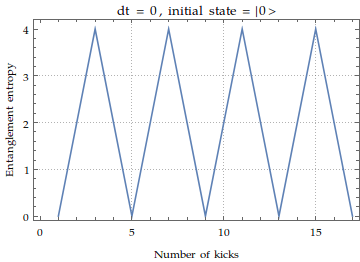
\includegraphics[scale=0.8,center]{dt0.png}
\caption{Starting with the initial state $|0\rangle$ in a 8-spin chain, entanglement entropy of the subsystem consisting of first 4 spins is being plotted with time for the case of periodic  driving. }
\label{normal}
\end{figure}
		 
		 
\section{Aperiodic Driving}
		
		Consider an aperiodic driving protocol where the kicking occurs after a time period with a probability p. The unitary operator acting for the n$^{th}$ time for this protocol will be: 
		
		\begin{equation}
		 U_n =  \exp(-i\dfrac{\pi}{4}\sum_{j=1}^{L}\sigma_{j}^{x} \sigma_{j+1}^{x})  \exp(-i\dfrac{\pi}{4}\sum_{j=1}^{L}\sigma_{j}^{z})^{\alpha_n}\, , \quad \alpha_n \epsilon \{0,1\}
		 \end{equation}
		
\section{Jordan Wigner Transformations}

Performing Jordan-Wigner transformations to the interaction and magnetic field terms in the Hamiltonian, it takes the following form when expressed in the space of fermion-momentum modes: 

	\begin{align}
			H_{kick} &= 2 \sum_{k}  [d_{k}^\dagger d_{k} - d_{-k}^\dagger d_{-k}]\\
			H_{after} &= -2\sum_{k}(  \cos k [d_{k}^\dagger d_{k} - d_{-k}^\dagger d_{-k}] -  \sin k [d_{-k}d_{k} + d_{k}^\dagger d_{-k}^\dagger])
			\end{align}	
		 
	Now let us define a new space whose basis states are $ |0\rangle $ (which is the no fermion state in the momentum basis) and $ d_{k}^\dagger d_{-k}^\dagger |0\rangle $. Hamiltonian takes this simple form in this basis:
			
			\begin{align}
			H_{kick} &= -2 \sum_{k}  \sigma_{k}^z\\
			H_{after} &= 2\sum_{k} (\cos k \sigma_{k}^z - \sin k \sigma_{k}^x )
			\end{align}	
			
			
	The initial state is taken to be the ground state of the interaction Hamiltonian. In this newly defined basis, it takes the following form:
		
		\begin{equation}\label{key}
		 |\psi(0)\rangle_{k} = v_{k}(0) |0\rangle + u_{k}(0) |1\rangle
		\end{equation}
		
		Where $ v_{k}(0) = \sin(k/2) $ and $ u_{k}(0) = \cos(k/2) $
		
		Now the unitary evolution of this initial state is: 
		
		\begin{equation}\label{key}
		i \dfrac{d}{dt} \begin{bmatrix}
		v_{k}(t)\\u_{k}(t)
		\end{bmatrix} =  H_{k}\begin{bmatrix}
			v_{k}(t)\\u_{k}(t)
		\end{bmatrix}
		\end{equation}
		
		Now since $ H_{k} $ is in the form of  2 x 2  matrices, the numerical computation of the evolution of the states becomes exponentially faster. 
 		
 		Lets us see what the Floquet operator looks like in this case, for the particular case where the time period is $ \dfrac{\pi}{4} $: 
 		
 			\begin{align}
 		U_{kick}& = \exp(-i \dfrac{\pi}{4} H_{kick})\\
 		& = \exp(i \dfrac{\pi}{2} \sum_{k}\sigma_{k}^z)\\
 		& = i\prod_{\otimes k} \sigma_{k}^z\\
 		U_{after} & = \exp(-i\dfrac{\pi}{4}H_{after})\\
 		&= \exp(-i\dfrac{\pi}{2}\sum_{k} (\cos k \sigma_{k}^z - \sin k \sigma_{k}^x ))\\
 		& = -i \prod_{\otimes k} (\cos k \sigma_{k}^z - \sin k \sigma_{k}^x )
 		\end{align}
 		
 	In the presence of no noise, the Floquet operator takes the simple form: 
 	
 	\begin{equation}\label{key}
 	U = - \prod_{\otimes k} (\cos k - \sin k \sigma_{k}^x \sigma_{k}^z)
  	\end{equation}
  	
  	Note that this simple expression for the Floquet operator occurs only for the case when the period of the kicks happens to be $ \pi/4 $ which is a special case where the system sees symmetries. 
  	
  	
  	In the presence of noise, the unitary operator for the kth mode  turns out to be (with $ \epsilon $ being 0 or 1 with a probability of 1/2 ) and $ U_{j} $  the unitary operator acting after $ j $ periods\cite{PhysRevB.98.064305}: 
  	
  	\begin{align}
  	U_{kick} &= (i\sigma_{k}^z)^\epsilon\\
  	U_{after}& =  -i  (\cos k \sigma_{k}^z - \sin k \sigma_{k}^x )
  	\end{align}
  	
  	\begin{align}
  	U_{j} &=   \begin{bmatrix}
  	\cos k & -\sin k\\
  	-\sin k & -\cos k \\ 
  	\end{bmatrix} \begin{bmatrix}
  	1& 0 \\
  	0 & (-1)^{\epsilon_{j}}\\
  	\end{bmatrix} =  \begin{bmatrix}
  	\cos k & -(-1)^{\epsilon_{j}}\sin k \\
  	-\sin k & -(-1)^{\epsilon_{j}}\cos k \\  
  	\end{bmatrix}\\
   	U_{j}U_{l} 	&=  \begin{bmatrix}
  	\cos k & -(-1)^{\epsilon_{j}}\sin k \\
  	-\sin k & -(-1)^{\epsilon_{j}}\cos k \\  
  	\end{bmatrix}  \begin{bmatrix}
  	\cos k & -(-1)^{\epsilon_{l}}\sin k \\
  	-\sin k & -(-1)^{\epsilon_{l}}\cos k \\  
  	\end{bmatrix}\\
  	& = \begin{bmatrix}
  	\cos^2 k + (-1)^{\epsilon_{j}}\sin^2 k & \cos k \sin k(-(-1)^{\epsilon_{j}} + (-1)^{\epsilon_{j}+\epsilon_{l}})\\
  	\sin k \cos k (-1 + (-1)^{\epsilon_{j}})& (-1)^{\epsilon_{l}}\sin^2 k + (-1)^{\epsilon_{j}+\epsilon_{l}}\cos^2  k\\
  	\end{bmatrix}
    	\end{align}
 	
 		\subsection[Geometric picture]{Visualizing k-mode evolution on the Bloch sphere}
		
		Now that we have $ \begin{bmatrix}
		v_{k}(t)\\u_{k}(t)
		\end{bmatrix} $ for any t, we would want to visualize this time evolution on the Bloch sphere. 
		
		Consider a single k-mode:
		
		\begin{align}
		\begin{bmatrix}
		v_{k}(t)\\u_{k}(t)
		\end{bmatrix}  & = e^{i\beta} \cos[\dfrac{\theta}{2}] |0\rangle + e^{i\alpha} \sin[\dfrac{\theta}{2}] |1\rangle \\
		&=   e^{i\beta}(\cos[\dfrac{\theta}{2}] |0\rangle + e^{i(\alpha-\beta)} \sin[\dfrac{\theta}{2}] |1\rangle)
		\end{align}
		
		
		
		
		Now we need to find out $ \theta  $ and $ (\alpha-\beta) $. This can be found out from the following constraints. 
		
		\begin{align}
		|v_{k}|^2 + |u_{k}|^2 &= 1  \\ 
		\theta & = 2 \cos^{-1} (|v_k|)	\\
		e^{i\beta} = v_k/\cos(\theta/2)	\\
		e^{i(\alpha-\beta)} = \dfrac{u_k}{v_k} \cot(\theta/2)
				\end{align}
				
				
		With the parameters $ \theta  \text{and} (\alpha - \beta) $ know, we can now plot the k-mode evolution on the Bloch sphere. Notice that in this special case where the time period is taken to be $ \pi/4 $ the action of the Floquet operator does not bring about any change to the relative phase i.e., $ (\alpha- \beta) $. We start off with the initial state whose parameters $ \theta_{0}$ and $\phi_{0} = (\alpha_{0} - \beta_{0}) $ are known. 
		
		\begin{figure}
			\centering
			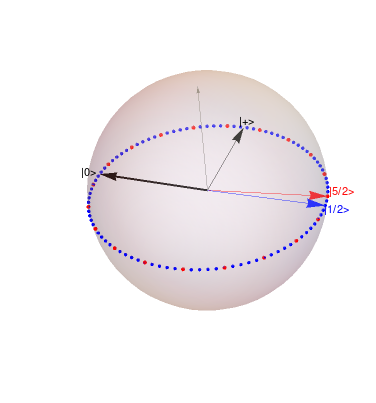
\includegraphics[width=0.7\linewidth]{piby4blochsphere}
			\caption{k-mode evolution, when  $T = \pi/4 $. The colored arrow shows the initial states for two modes $ k  = \pi/100 $ and $ k = 5\pi/100 $ }
			\label{fig:piby4blochsphere}
		\end{figure}
	
	\begin{figure}
		\centering
		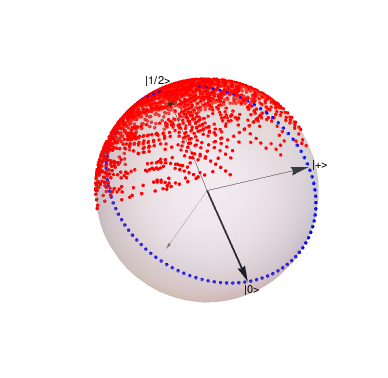
\includegraphics[width=0.5\linewidth]{blochsphere_half_01}
		\caption{k-mode evolution, when  $T = \pi/4 + 0.01 $ shown  in red for  $ k  = \pi/100 $ and the blue points correspond to $ T = \pi/4 $}
		\label{fig:blochspherehalf01}
	\end{figure}
	\begin{figure}
		\centering
		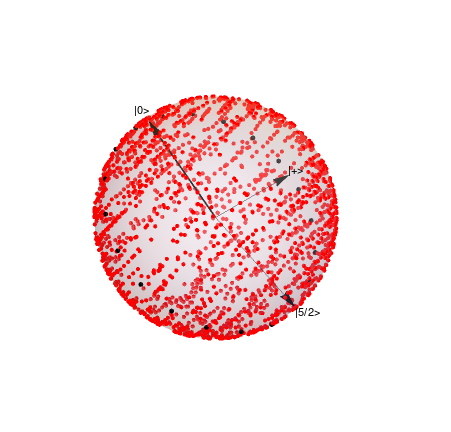
\includegraphics[width=0.5\linewidth]{blochsphere_fiveby2_01}
		\caption{k-mode evolution, when  $T = \pi/4 + 0.01 $ shown  in red for  $ k  = 5\pi/100 $ and the blue points correspond to $ T = \pi/4 $}
		\label{fig:blochspherefiveby201}
	\end{figure}
	
	\subsection{Entanglement Entropy of the fermion subsystem}
		
		The entanglement entropy of the subsystem can be evaluated by calculating the Von Neumann entropy of the reduced density matrix of the subsystem. While dealing with fermionic systems, it can be shown that 
		
\subsubsection{Calculating Reduced density matrix from correlation functions}		

Any density matrix can be expressed as:

\begin{equation}\label{rho_exp}
\rho = \dfrac{1}{\mathcal{Z}}\exp(-\beta \mathcal{H})
\end{equation}

Where $ \mathcal{H} $ is a Hermitian matrix, $ \beta $ is a constant and $ \mathcal{Z} $ is the normalization factor (partition function). This way of expression can be justified by noting that $ \rho $ is always positive definite and $ Tr[\rho] = 1 $, and Eq.\eqref{rho_exp} satisfies both these conditions. 

Any general Hermititan operator for a system comprising of N 2-state particles can be written in terms of Pauli matrices and Identity operator as:

\begin{equation}\label{key}
\mathcal{H} = \prod_{\otimes k}(\vec{B_{k}}\cdot\vec{\sigma}+\mu_{k}\mathcal{I})
\end{equation} 

In the case of free fermions hopping between lattices the Hamiltonian has the form: 

\begin{equation}\label{key}
\hat{H}  = - \sum_{n,m} \hat{t}_{nm}c_{n}^\dagger c_{m}
\end{equation}

The reduced density matrix of a subsystem with $ M $ sites formed by the combination of eigenvectors of the above Hamiltonian can be expressed in the following form:

\begin{equation}\label{key}
\rho  = \dfrac{1}{\mathcal{Z}} \exp(-\sum_{i,j}H_{ij}c_{i}^\dagger c_{j})
\end{equation}

Let us denote $ \mathcal{H} = -\sum_{i,j}H_{ij}c_{i}^\dagger c_{j}  $. 

Diagonalizing $ \mathcal{H} $ by exploiting its eigenvectors $ \phi_{k} $ and eigenvalues $ \epsilon_{k} $   such that 

\begin{equation}\label{key}
c_{i} = \sum_{k} \phi_{k}(i) a_{k}
\end{equation}

Now $ \rho $ becomes 

\begin{equation}\label{kedy}
\rho  = \dfrac{1}{\mathcal{Z}} \exp(-\sum_{k = 1}^{M}\epsilon_{k}a_{k}^\dagger a_{k})
\end{equation}

Now consider the correlation matrix given by:

\begin{equation}
\hat{C}_{mn} = \langle c_{m}^\dagger c_{n}\rangle
\end{equation}



By exploiting the properties of free fermion system, we can note that:

\begin{equation}
\langle c_{n}^\dagger c_{m}^\dagger c_{k}c_{l}\rangle = \langle c_{n}^\dagger c_{l}\rangle \langle c_{m}^\dagger c_{k}\rangle-\langle c_{n}^\dagger c_{k}\rangle \langle c_{m}^\dagger c_{l}\rangle
\end{equation}

We know that:
\begin{equation}
\langle c_{m}^\dagger c_{n}\rangle = Tr[\rho c_{m}^\dagger c_{n}]
\end{equation}

Now the problem is to find the reduced density matrix using the correlation functions. From Wick's theorem, $\rho$ can be decribed in terms of fermions as follows:

\begin{equation}
\rho = K e^{-\sum_{i,j}H_{ij}c_{i}^\dagger c_{j}}
\end{equation}

Diagonalizng the $H$ matrix with its eigen values being $\epsilon_{k}$ with eigen functions being $ \phi_{k} (i)$. The diagonalizaiton process is done in the following way:

\begin{equation}
c_{i} = \sum_{k}\phi_{k}(i)a_{k}
\end{equation}

With this the density matrix now becomes:

\begin{equation}
\rho = K e^{-\sum_{k}\epsilon_{k}a_{k}^\dagger a_{k}}
\end{equation}

Finally the eigen values $\chi_{k}$ of $\hat{C}$ and $\epsilon_{k}$ of $H$ are related by:

\begin{equation}
\chi_{k}  =(e^{\epsilon_{k}} +1)^{-1}
\end{equation}

In matrix form:

\begin{equation}
H^T = \ln [(1-C)/C]
\end{equation}
		
		Therefore $\rho $ can be comlpetely determined once $\hat{C}$ is known. 
	
Now consider the case of kicked Ising chain. Correlation matrix in this case after Fourier transforming the fermion operators is given by: 
		
		\begin{align}
		D_{kl} &= \langle d_{k}^\dagger d_{l} \rangle =\dfrac{1}{N} \langle \sum_{m} e^{ikm} c_{m}^\dagger\sum_{n} e^{-iln}c_{n}\rangle \\
		D_{kl} &= \dfrac{1}{N}\sum_{m,n} e^{i\pi(mk-nl)/N}C_{mn}\\
		C_{mn}&=  \dfrac{1}{N}\sum_{k,l} e^{-i\pi(mk-nl)/N}D_{kl}
		\end{align}
		
		Given that the unitary operator is given by \ref{noisyunitary} the state is evolved in the $d_{k}$ basis. The correlation matrix $\hat{C}$ can be calculated by taking the Fourier transform of the correlation matrix in $d_{k}$ basis. 
Let the initial state be defined to be $|\psi(0)\rangle$ the state after N kicks is given by $U^N |\psi(0)\rangle$. The correlation matrix after N kicks happens to be :

\begin{align}
D_{mn}(N) &= \dfrac{1}{N} \langle \psi(0)|U^{\dagger N} d_{m}^\dagger d_{n}  U^{ N}| \psi(0)\rangle\\
C_{mn}(N) &= \dfrac{1}{N} \sum_{k,l} e^{-i\pi(mk-nl)/N} \langle \psi(0)|U^{\dagger N} d_{k}^\dagger d_{l}  U^{ N}| \psi(0)\rangle
\end{align}		


Another correlation matrix, $ F $ is defined as:

\begin{equation}\label{key}
F_{mn}(N) = \dfrac{1}{N} \sum_{k,l} e^{-i\pi(mk+nl)/N} \langle \psi(0)|U^{\dagger N} d_{k}^\dagger d_{l}^\dagger  U^{ N}| \psi(0)\rangle
\end{equation}

Taking into account both these correlation matrices, the $ 2l \times 2l $ matrix $ \mathcal{C}[2l] $ is formed:

\begin{equation}\label{key}
\mathcal{C} = \begin{bmatrix}
I - C & F\\
F^\dagger & C\\
\end{bmatrix}
\end{equation}

So this was done for the reduced density matrix in the fermion space. How can we correlate to the reduced density matrix in the spin space? 


 
\textbf{Claim} : Von Neumann entropy of the eigen values of $ \mathcal{C}  $ is the same as the Von Neumann entropy of the reduced density matrix of the subsystem of length $ l $. With this, the correlation matrix can be easily calculated and we can obtain the entanglement entropy.


\begin{figure}
	\centering
	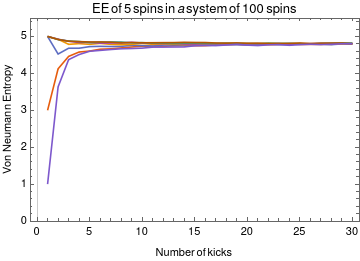
\includegraphics[width=0.7\linewidth]{5_95_EE}
	\caption{}
	\label{fig:595ee}
\end{figure}
\begin{figure}
	\centering
	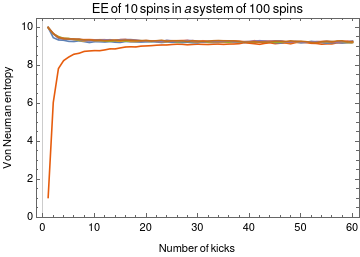
\includegraphics[width=0.7\linewidth]{10_90_EE}
	\caption{}
	\label{fig:1090ee}
\end{figure}

\begin{section}{Remarks}
	\begin{itemize}
		\item Eigen value spectra of the reduced density matrix needs to be calculated in order to look for signs of quantum chaos and thermalization
		\item Aperiodicity along the lines of Thue Morse, Fibonacci sequences also shows interesting entanglement behaviour. 
	\end{itemize}
\end{section}

		
 	
 			 
		 
	\bibliographystyle{plain}
	\bibliography{references}
	
\end{document}